%%%%%%%%%%%%%%%%%%%%%%%%%%%%%%%%%%%%%%%%%
% University Assignment Title Page 
% LaTeX Template
%
% This template has been downloaded from:
% http://www.latextemplates.com
%
% Original author:
% WikiBooks (http://en.wikibooks.org/wiki/LaTeX/Title_Creation)
% 
% Instructions for using this template:
% This title page is presently capable of being compiled as is. This is not 
% useful for including it in another document. To do this, you have two options: 
%
% 1) Copy/paste everything between \begin{document} and \end{document} 
% starting at \begin{titlepage} and paste this into another LaTeX file where you 
% want your title page.
% OR
% 2) Remove everything outside the \begin{titlepage} and \end{titlepage} and 
% move this file to the same directory as the LaTeX file you wish to add it to. 
% Then add \input{./title_page_1.tex} to your LaTeX file where you want your
% title page.
%
%%%%%%%%%%%%%%%%%%%%%%%%%%%%%%%%%%%%%%%%%

%----------------------------------------------------------------------------------------
%	PACKAGES AND OTHER DOCUMENT CONFIGURATIONS
%----------------------------------------------------------------------------------------

\documentclass[12pt]{article}
\usepackage[utf8]{inputenc}
\usepackage[francais]{babel}
\usepackage{graphicx}
\graphicspath{{./Screenshots/}}

\begin{document}

\begin{titlepage}

\newcommand{\HRule}{\rule{\linewidth}{0.5mm}} % Defines a new command for the horizontal lines, change thickness here

\center % Center everything on the page
 
%----------------------------------------------------------------------------------------
%	HEADING SECTIONS
%----------------------------------------------------------------------------------------

\textsc{\LARGE INSA de Rennes}\\[1.5cm] % Name of your university/college
\textsc{\Large Programmation Orientée Objet}\\[0.5cm] % Major heading such as course name
\textsc{\large Projet C++}\\[0.5cm] % Minor heading such as course title

%----------------------------------------------------------------------------------------
%	TITLE SECTION
%----------------------------------------------------------------------------------------

\HRule \\[0.4cm]
{ \huge \bfseries Rapport de conception}\\[0.4cm] % Title of your document
\HRule \\[1.5cm]
 
%----------------------------------------------------------------------------------------
%	AUTHOR SECTION
%----------------------------------------------------------------------------------------

\begin{minipage}{0.4\textwidth}
\begin{flushleft} \large
\emph{Author:}\\
Jean \textsc{Guegant}\\ % Your name
Richard \textsc{Lagrange} % Your name
\end{flushleft}
\end{minipage}
~
\begin{minipage}{0.4\textwidth}
\begin{flushright} \large
\emph{Supervisor:} \\
Alexandru \textsc{Costan} % Supervisor's Name
\end{flushright}
\end{minipage}\\[4cm]

% If you don't want a supervisor, uncomment the two lines below and remove the section above
%\Large \emph{Author:}\\
%John \textsc{Smith}\\[3cm] % Your name

%----------------------------------------------------------------------------------------
%	DATE SECTION
%----------------------------------------------------------------------------------------

{\large \today}\\[3cm] % Date, change the \today to a set date if you want to be precise

%----------------------------------------------------------------------------------------
%	LOGO SECTION
%----------------------------------------------------------------------------------------

%\includegraphics{Logo}\\[1cm] % Include a department/university logo - this will require the graphicx package
 
%----------------------------------------------------------------------------------------

\vfill % Fill the rest of the page with whitespace

\end{titlepage}

\tableofcontents{}

\section{Introduction}

	Lors de la modélisation de notre version de \textit{Civilization}, nous avons voulu rendre notre code le plus flexible et extensible possible.
Nous voulions pouvoir facilement ajouter la gestion des jeux en réseau, pouvoir étendre et créer ses propres classes, etc.
Heureusement, ceci est réalisable grâce aux \textit{design patterns} (qui nous sont aussi imposés).
Nous avons essayé d'aller plus loin que les 5 patrons de conceptions imposé, afin de réaliser notre objectif d'un jeu pouvant évoluer. Nous justifierons nos différents choix techniques tout au long de ce rapport.
Bonne lecture.

\newpage

\section{Diagrammes de cas d'utilisation}
	\subsection{Règles du jeu}
		Dans ce diagramme, nous avons illustré les intéractions entre les concepts du jeu et les joueurs. (Schéma \ref{oldciv})
	Les joueurs sont ceux qui créent des villes, créent des unités, bougent, font combattre les unités et capturent des villes.
	Les dépendances entre les entités du jeu apparaissent le plus clairement possible.
	
	\subsection{Cycle de vie d'une partie}
	Ce diagramme illustre toutes les phases du logiciel, avec les choix potentiels des joueurs.(Schéma \ref{cyclevie})
	
\section{Diagrammes de Classe}
Nous avons commencé par modéliser l'ensemble des interfaces des entités que nous voudrions manipuler. Ceci nous a permis de ce concentrer sur l'interaction des objets sans se préoccuper de leurs implémentations. Par la suite, nous avons implémenté les différentes interfaces par des classes concrètes. A noter que dans certains cas particulier nous avons regroupé interface et une partie de l'implémentation sous forme de classe abstraite. Ci-dessous vous trouverez les différents les diagrammes de classes finaux de notre application regroupées par espace de noms. 
	\subsection{Civilization : schéma \ref{civ}}
		\subsubsection{Namespace Civilization}
			Nous avons utilisé le design pattern Prototype pour pouvoir avoir le plus possible de civilizations différentes.
		En effet, au départ nous étions partis sur le patron de conception Fabrique Abstraite classique, ce qui aurait donné le Schéma 3. C'est à dire implémenter une classe concrète pour chacune des civilisations.
			Après réflexion, nous voulions pouvoir étendre facilement le nombre de civilisations (tout joueur n'est pas forcement suffisamment émérite en C\# pour pouvoir rajouter sa propre classe).
		Le joueur pourrait importer sa civilisation créée, sous forme d'un fichier XML par exemple. 
		Donc pour implémenter cette solution, nous avons utilisé une Fabrique Concrète utilisant des prototypes d'unités différents à cloner lorsqu'il désire utiliser telle ou telle civilisation. (Schéma 4)
		Cette Fabrique Concrète a donc un constructeur qui a comme rôle de récupérer des unités clonables spécifiques à une civilisation (Directeur, étudiant, etc.), pour en fabriquer d'autres, avec des caractéristiques uniques.
Ces instances particulières des unités peuvent provenir de 2 endroits :
\begin{enumerate}
\item Soit l'utilisateur les a crée lui même, via une interface utilisateur, qui créera un fichier XML contenant le prototype unité sérialisé (l'interface ISerializable de C\# permet de définir cette possibilité de sérialisation).
\item Soit ce sont des unités prédéfinies que l'on aura créées auparavant. (Il faudra alors désérialiser l'unité prototype, qui est stockée sous la forme d'un fichier XML comme pour la 1ère méthode.)
\end{enumerate}
		Le couplage du pattern Fabrique Abstraite avec le pattern prototype nous permet d'éviter un nombre de sous-classes important. Toutefois il est toujours possible de coder des civilisations en dur en implémentant un autre type de fabrique concrète.

		
		\subsubsection{Namespace Unit}
			Une interface commune IUnit est pratique dans le cas où l'on déciderais de faire une unité qui a une attaque qui dépend de plusieurs facteurs.
		(Comme par exemple : attaque = attaque de base + attaque de l'épée + attaque du compagnon). Une interface commune permet de réaliser ceci facilement.
			La classe Unit est \textit{ISerializable} (comme expliqué auparavant) et \textit{IDrawable} (pour avoir les méthodes d'affichage).
		On a aussi des interfaces spécifiques pour les types d'unités spéciales (IDirector, IStudent, ITeacher), ce qui nous donne une certaine flexibilité.
			Si jamais l'on décide de changer la gestion des bonus des directeurs de département par exemple, cette interface permettra de le changer sans toucher au code client.
		
		\subsubsection{Namespace City}
			De même que pour IUnit, nous avons pensé à une interface ICity (qui pourrait se revéler pratique si nous voulons étendre un autre concept à des villes de type différent).
		Par exmple, nous pourrions imaginer une ville dont \textit{TotalAvailableFood} dépend aussi de son commerce avec une autre ville par exemple, nous pouvons changer la manière dont est implémenté cette méthode à chaud sans risquer de changer le code client.
			Ensuite, nous avons utilisé le pattern Stratégie afin d'implémenter des algorithmes différents d'extension de la ville (\textit{"Le choix de cette case, sera réalisé par un algorithme que vous développerez."})
		Ainsi, on pourra au départ implémenter un algorithme simple et bête qui choisira une case aléatoirement.
			Puis dans un deuxième temps, choisir d'implémenter un algorithme plus intelligent, qui choisira les case en fonction de leur contenu exploitable (minerai, nourriture).
		De plus, vu qu'une seule instance de cet algorithme est utile à la fois, nous utiliseront le patron de conception Singleton (le pattern Singleton se retrouve dans toutes les patterns algorithme de notre projet).
			
	
	\subsection{View : schéma \ref{view}}
		\subsubsection{Namespace Drawable} 
			TileFlyWeight est un pattern poids-mouche (flyweight) pour les tiles (textures) que nous allons utiliser pour la vue de notre jeu.
		En effet, de nombreuses cases de la carte de notre jeu ainsi que les différentes unités utilisent les mêmes textures. Afin d'éviter d'encombrer
		inutilement la mémoire en chargeant plusieurs fois la même texture, nous allons partager une même instance de cette texture aux différents objets la nécessitant.
		Pour cela, notre pattern flyweight contient une hashmap liant un nom de texture à son contenu. 
		Par exemple si plusieurs objets demandent le tile "water.png", ceux-ci partageront une unique instance du tile "water.png". 
		A noter que si aucun objet ne demande "water.png", la texture ne sera jamais chargé en mémoire.
			On pourrait se demander si il n'est pas plus judicieux de partager les objets cases de notre carte et pas uniquement leurs textures. 
		En effet nous pourrions décider que toutes les cases "moutain" soit partagées car elles contiennent les mêmes caractéristiques 
		(hormis leur position, une caractéristique qui serait alors passé en état externe lors des manipulations).
			Nous projetons de créer des cases avec des caractéristiques variant au cours du temps (par exemple, la nourriture diminue en cas de guerre de proche), 
		il est alors difficile envisageable de contenir toutes les caractéristiques en état externe. C'est dans cette optique que nous ne partageons uniquement les textures des cases.
		Notre poids-mouche est un singleton car il n'y aucune raison de l'instancier plusieurs fois au cours d'une même partie.
		(hormis leur position, une caractéristique qui serait alors passé en état externe lors des manipulations).
			Nous projetons de créer des cases avec des caractéristiques variant au cours du temps (par exemple, la nourriture diminue en cas de guerre de proche), 
		il est alors difficile envisageable de contenir toutes les caractéristiques en état externe. C'est dans cette optique que nous ne partageons uniquement les textures des cases.
		Notre poids-mouche est un singleton car il n'y aucune raison de l'instancier plusieurs fois au cours d'une même partie.
		\paragraph{}
		La classe Tile a son constructeur privé car nous voulons que les Tiles soit chargés uniquement à partir du FlyWeight. 
		On remarquera également que la méthode \textit{Draw} prend un paramètre d'état externe qui est la position du tile que nous voulons dessiner 
		(comme vu précédemment le pattern FlyWeight oblige à passer les états non-partagés d'un objet à l'aide de paramètres externes).
		\paragraph{}
		Nous avons mit à la disposition des développeurs une interface ISprite pour dessiner des animations. Un sprite consistant en une série de textures que l'on fait défiler afin de donner l'illusion 
		d'une animation. L'implémentation de cette interface est faite avec la classe Sprite qui gère des animations basiques. Encore une fois l'intérêt d'une interface ISprite est de pouvoir facilement changer l'implémentation
		sans réécrire tout le code client.
		\paragraph{}
		Pour la vue, nous avons également l'interface IDrawable qui doit être implémenté par toutes les entités que nous voudrons dessiner (les cases, les unités, ...). 
		Cette interface contient deux fonctions :
		\begin{itemize}		
		\item Draw qui permet de dessiner l'entité, le paramètre IGraphiqueEngine sera détaillé par la suite.
		\item Update qui met à jour l'état graphique de l'entité que nous allons dessiner. En effet, si nous utilisons des animations, il est important de modifier l'état de la prochaine frame que nous allons dessiner.
		Le paramètre deltaTime est la différence de temps entre la frame précédente et la frame courante. Nous exprimeront l'ensemble de nos animations à l'aide de ce paramètre, ainsi peu importe la puissance de la machine
		sur laquelle tourne le jeu, les animations seront toujours de même durée et donc fluides.
		\end{itemize}
		\paragraph{}
			Nous espérons implémenter par la suite un pattern bridge pour séparer l'interface de notre moteur graphique de son implémentation. 
		En effet, il serait élégant de pouvoir faire tourner notre jeu en dehors de l'environnent WPF (XNA, DirectX, OpenGL par exemple).
		Pour cela nous avons imaginé une interface IGraphicEngine qui contiendra les appels graphiques nécéssaires au fonctionnement de notre jeux (DrawSprite, CreateSprite, LoadTile, ...).
		L'implémentation dans le cas de WPF est la classe WPFGraphicEngine, pour XNA se sera XNAGraphicEngine, ...
		Dans toutes les librairies graphiques nous retrouvons des appels à des primitives graphiques identiques(DrawTexture, LoadPNGTexture, ...). 
			L'interface IGraphicEngine dépend donc de son implémentation bas-niveau qui est l'interface IGraphicPrimitive qui contient l'ensemble de ces appels primitifs.
		Pour WPF nous créons alors une classe WPFGraphicPrimitive pour implémenter cette interface IGraphicPrimitive. Il en va des même pour les autres environnements que nous détirons utiliser.
		Ce pattern bridge ne contient pour l'instant aucune méthode car nous ne sommes pas encore certains des fonctions graphiques nécessaires à notre jeu.

		
	\subsection{World : schéma \ref{world}}
		\subsubsection{Namespace World}
			\subsubsection{Namespace Square}
				Dans le namespace Square, nous avons créé une classe pour représenter une case du "damier" de notre jeu.
			Ces cases peuvent être de natures différentes (Montagne, Plaine, Désert) et avoir des ressources spéciales (Fer, Fruit).
			Grâce à ces natures et ressources spéciales, on peut avoir de nombreux types de cases différents.
			Une implémentation idéale de ce cas serait le patron de conception Décorateur.
			En effet, grâce au décorateur, on peut alors "décorer" les cases Montagne, Plaine ou Désert avec les ressources spéciales Fer et Fruit.
			Il est aussi facile d'ajouter une nature ou une ressource spéciales, sans tout de même faire exploser le nombre de classes filles.
			
			\subsubsection{Namespace Map}
				L'interface IMapCreate permet d'obliger les classes de type SmallMap ou MediumMap qui l'implémentent d'avoir une méthode CreateMap. Cette architecture peut sembler étrange par la présence du paramètre randomizer.
			En fait, il s'agit du patron de conception Stratégie appliquée à une interface.
			Le lien entre l'interface IMapCreate et ISquareRandomizer n'est pas aussi fort qu'une agrégation, mais doit quand même avoir un randomizer passé en paramètre.
			Il est alors facile d'avoir des stratégies différentes de création de cartes, si on veut des cartes avec plus de mer par exemple, ou plus de montagne.
				Un autre patron de conception Stratégie se cache derrière SmallMap et MediumMap. La fonction \textit{CreateMap} renvoie une Map, qui sera différente en fonction de la taille (en plus du randomizer).
			En effet, dans une grande carte on pourrait avoir plus de cases d'eau, chose qu'on ne pourrait se permettre d'avoir quand on a une petite carte.
	
	\subsection{Fight : schéma \ref{fight}}
		\subsubsection{Namespace Fight}
			Dans le Namespace Fight, nous avons encore une fois utilisé le patron de conception stratégie.
			Elle nous permet de choisir quel algorithme de combat utiliser.
			En effet, nous avons imaginé plusieurs algorithmes différents en fonction de différents paramètres :
			\begin{enumerate}
				\item Le combat avec un Directeur de département sur la case comme support.
				\item Le combat normal d'une unité contre une autre.
				\item Le combat dans une ville (des fortifications doivent sûrement apporter un avantage défensif).
			\end{enumerate}
			L'intérêt d'une interface IFight est que si l'on veut un combat entre des groupes d'unités (en non plus du 1v1), on pourra implémenter cette interface par une autre classe.
			On aurait alors les méthodes utiles comme \textit{addDefender()} ou \textit{addFighter()}, qui n'interdisent pas l'ajout de plusieurs unités.
		
	\subsection{Game : schéma \ref{game}}	
		\subsubsection{Namespace Game}
				Game est la classe centrale de notre jeu. 
				Nous pouvons la considérer comme un pattern médiateur car elle va gérer les communications (la logique) entre les objets de notre jeu.
			Cette classe implémente l'interface ISerializable afin de pouvoir enregistrer l'état de la partie dans un fichier de notre de choix et de pouvoir le recharger ultérieurement. Nous pourrons donc mettre à disposition un système de sauvegarde pour les joueurs. 
			La fonction MainLoop de notre classe Game est la boucle principale du jeu qui mettra à jour l'état de la partie puis dessinera celle-ci. 
			Si nous voulons changer le comportement de cette boucle, il est toujours possible d'étendre la classe Game et de redéfinir la fonction MainLoop.
				\paragraph{}
				Pour gérer les différentes phases du jeu, nous utiliserons le pattern State. 
			Pour cela nous avons créé l'interface IGameState qui contient des fonctions pour charger l'état courant, le démarrer, le stopper...
			La classe Game contient une pile d'état, l'état courant est alors l'état en sommet de pile. .
			En effet il est intéressant de garder l'état précédant pour pouvoir retourner facilement dans une phase précédente de la partie.
				\paragraph{}
				Pour lier les actions utilisateurs au modèle du jeu, nous utilisons le pattern observateur. Plus précisément, nous avons opté pour le système d'event de C\#	pour récupérer les mouvements de la souris et les actions du clavier dans les états de Game (respectivement les fonctions KeyboardPressedEventHandle,  MouseClickedEventHandler, MouseMovedEventHandler).
			
			\subsection{Player : schéma \ref{player}}
				\subsubsection{Namespace Player}
				Afin de pouvoir implémenter plusieurs types de joueurs, nous avons créé une interface commune IPlayer. 
				En effet nous voulons pouvoir gérer aussi bien un joueur humain qu'une intelligence artificielle, qu'un joueur en ligne, ...
				Nous avons pour l'instant deux implémentations :
					\begin{itemize}
					\item HumanPlayer : qui gère un joueur humain manipulant la machine sur laquelle tourne le jeu. 
Cette implémentation utilise, comme la classe Game, le pattern observateur pour gérer les entrées utilisateur (la souris et le clavier).
					\item AIPlayer : qui gère une intelligence artificielle basique.
					\end{itemize}
Les joueurs modifient le cours de la partie à l'aide d'une liste d'action qui est mise à jour à chaque tour.
Un joueur possède aussi un état (pattern state) qui influence son comportement. Par exemple un joueur peut être dans l'état actif, l'état inactif,
voire l'état déconnecté dans le cas d'un jeu en ligne. 
					
				\subsubsection{Namespace Player.Actions}
Nous avons décidé d'encapsuler les différentes actions des joueurs par un pattern commande. 
Les communications entre les objets sont donc maintenant contenues dans un objet ayant pour interface IPlayerAction.
On peut citer de nombreux avantages à utiliser ce pattern plutôt que des "appels bruts" à des fonctions :
\begin{itemize}
\item Loguer les différentes actions des joueurs.
\item Débuguer facilement le déroulement d'une partie.
\item Si l'on veut implémenter un système de replay, il nous suffira de loguer toutes les actions et de les rejouer.
\item Faire un système de retour en arrière.
\item Si l'on veut faire un jeu en ligne, il nous suffira d'envoyer les actions des joueurs par paquets sous forme sérializée. Il ne restera plus qu'à 
désérialiser les actions à la réception des paquets pour synchroniser les deux joueurs.
\end{itemize}

Pour l'instant nous implémentons cette interface à l'aide d'une classe InGameAction et de nombreuses sous-classes comme AttackAction, BuildCityAction, etc.
Nous envisageons de rajouter d'autres classes mères implémentant l'interface IPlayerAction, comme par exemple ChatBoxAction pour la gestion de dialogues.

\section{Diagramme d'états-transitions}
Nous avons créé deux diagrammes d'états-transitions :
\begin{itemize}
\item Un diagramme montrant la recherche d'un Tile dans le flyweight (voir schéma \ref{flyweight}).
\item Les états-transitions pour déplacer une unité(voir schéma \ref{dep}).
\end{itemize}

\section{Diagrammes d'interaction}
Nous avons créé deux diagrammes d'interaction :
\begin{itemize}
\item Un diagramme représentant le lancement d'une partie. Ce qui comprend la création d'une instance de la classe Game, la création d'une carte (Map), la création des deux joueurs et enfin la création du moteur graphique. Le jeu peut ensuite entrer dans l'état LoadingState, puis dans l'état ActiveGameState (la partie a alors commencé, voir schéma \ref{lancement}).
\item Un diagramme représentant une itération dans la boucle MainLoop. Cela consiste a dessiner toutes les unités de la map, a mettre à jour les animations pour la prochaine frame et enfin récupérer les actions du joueur actif. On voit dans ce diagramme que le joueur a décidé d'acheter une nouvelle unité Enseignant (voir schéma \ref{frame}).
\end{itemize}

\section{Annexes}
\begin{figure}
    \begin{center}  
    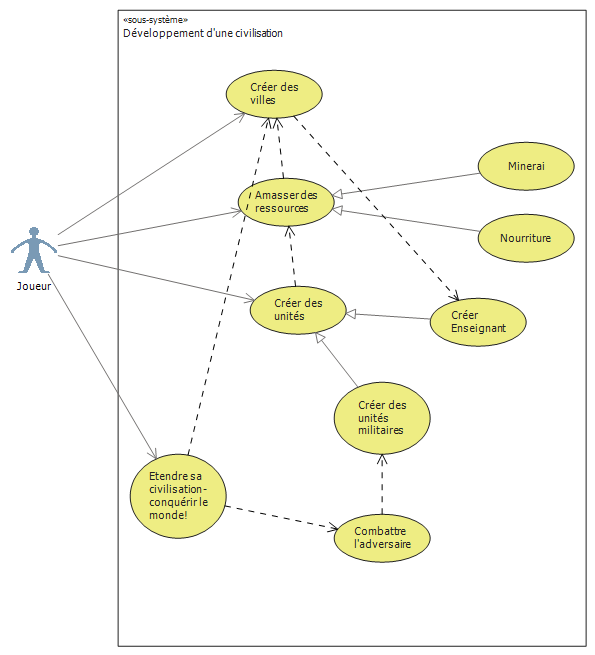
\includegraphics[width=\textwidth]{devci.png}
    \caption{Développement d'une civilisation.}
    \label{devci}
\end{center}
\end{figure}

\begin{figure}
    \begin{center}  
    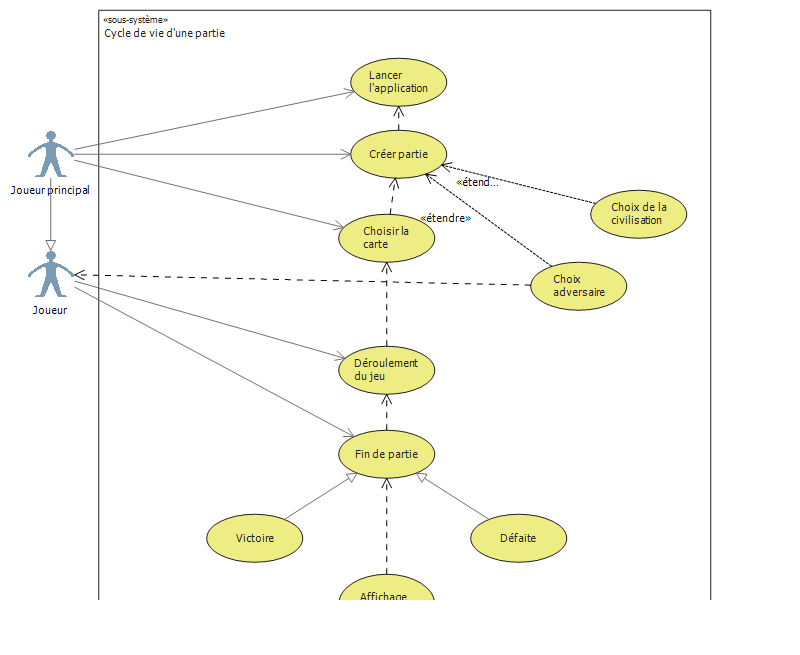
\includegraphics[width=\textwidth]{cyclevie.png}
    \caption{Cycle de vie d'une partie.}
    \label{cyclevie}
\end{center}
\end{figure}


\begin{figure}
    \begin{center}  
    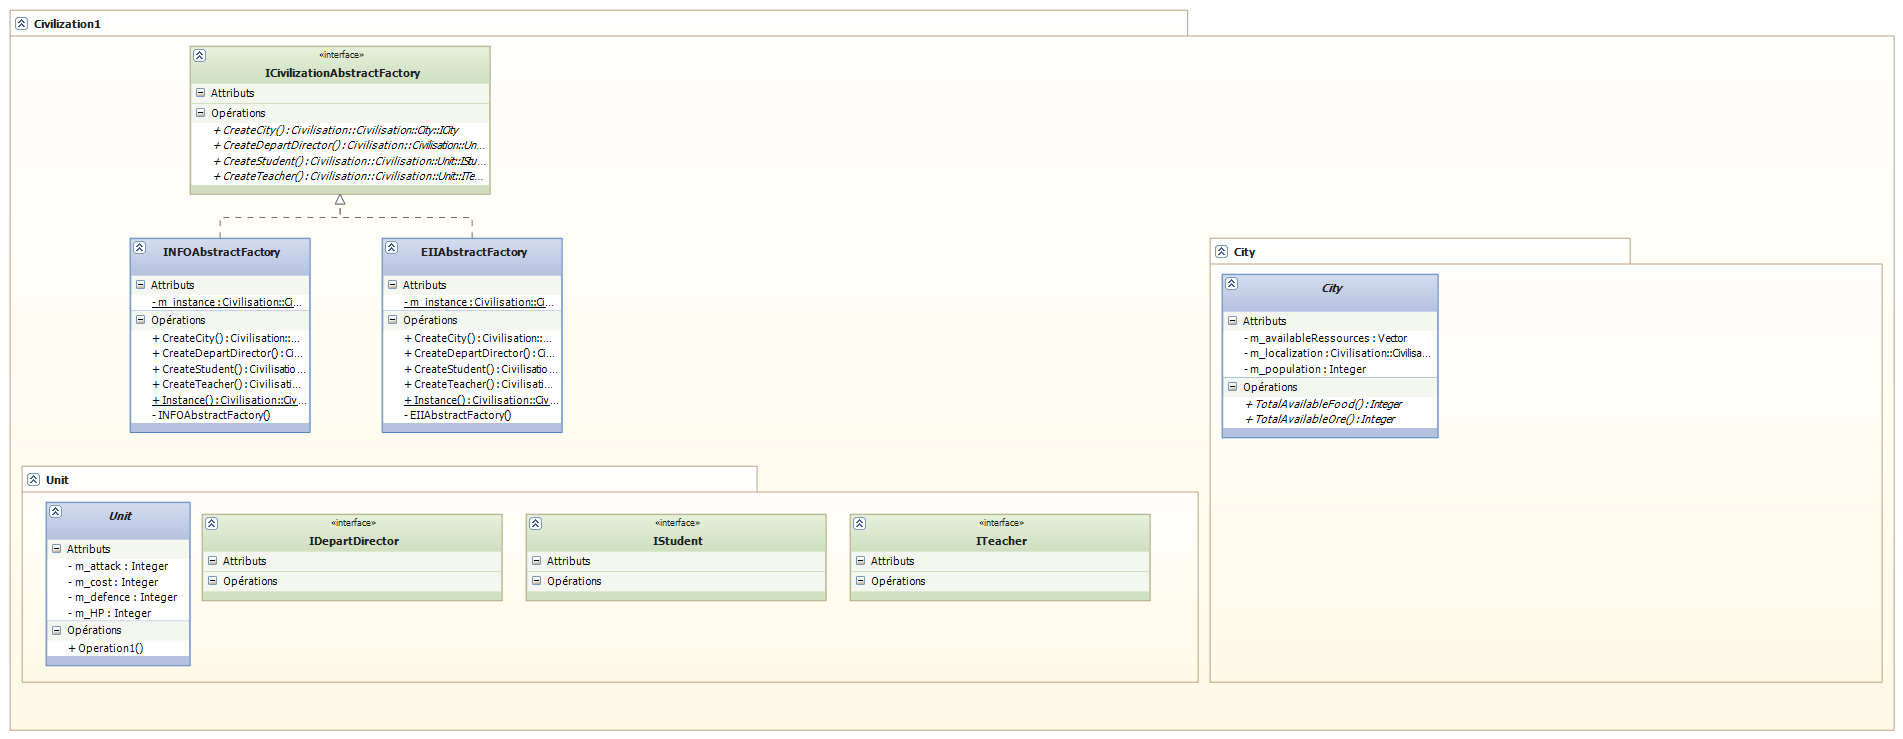
\includegraphics[width=\textwidth]{oldciv.png}
    \caption{Civilization (ancienne version).}
    \label{oldciv}
\end{center}
\end{figure}

\begin{figure}
    \begin{center}  
    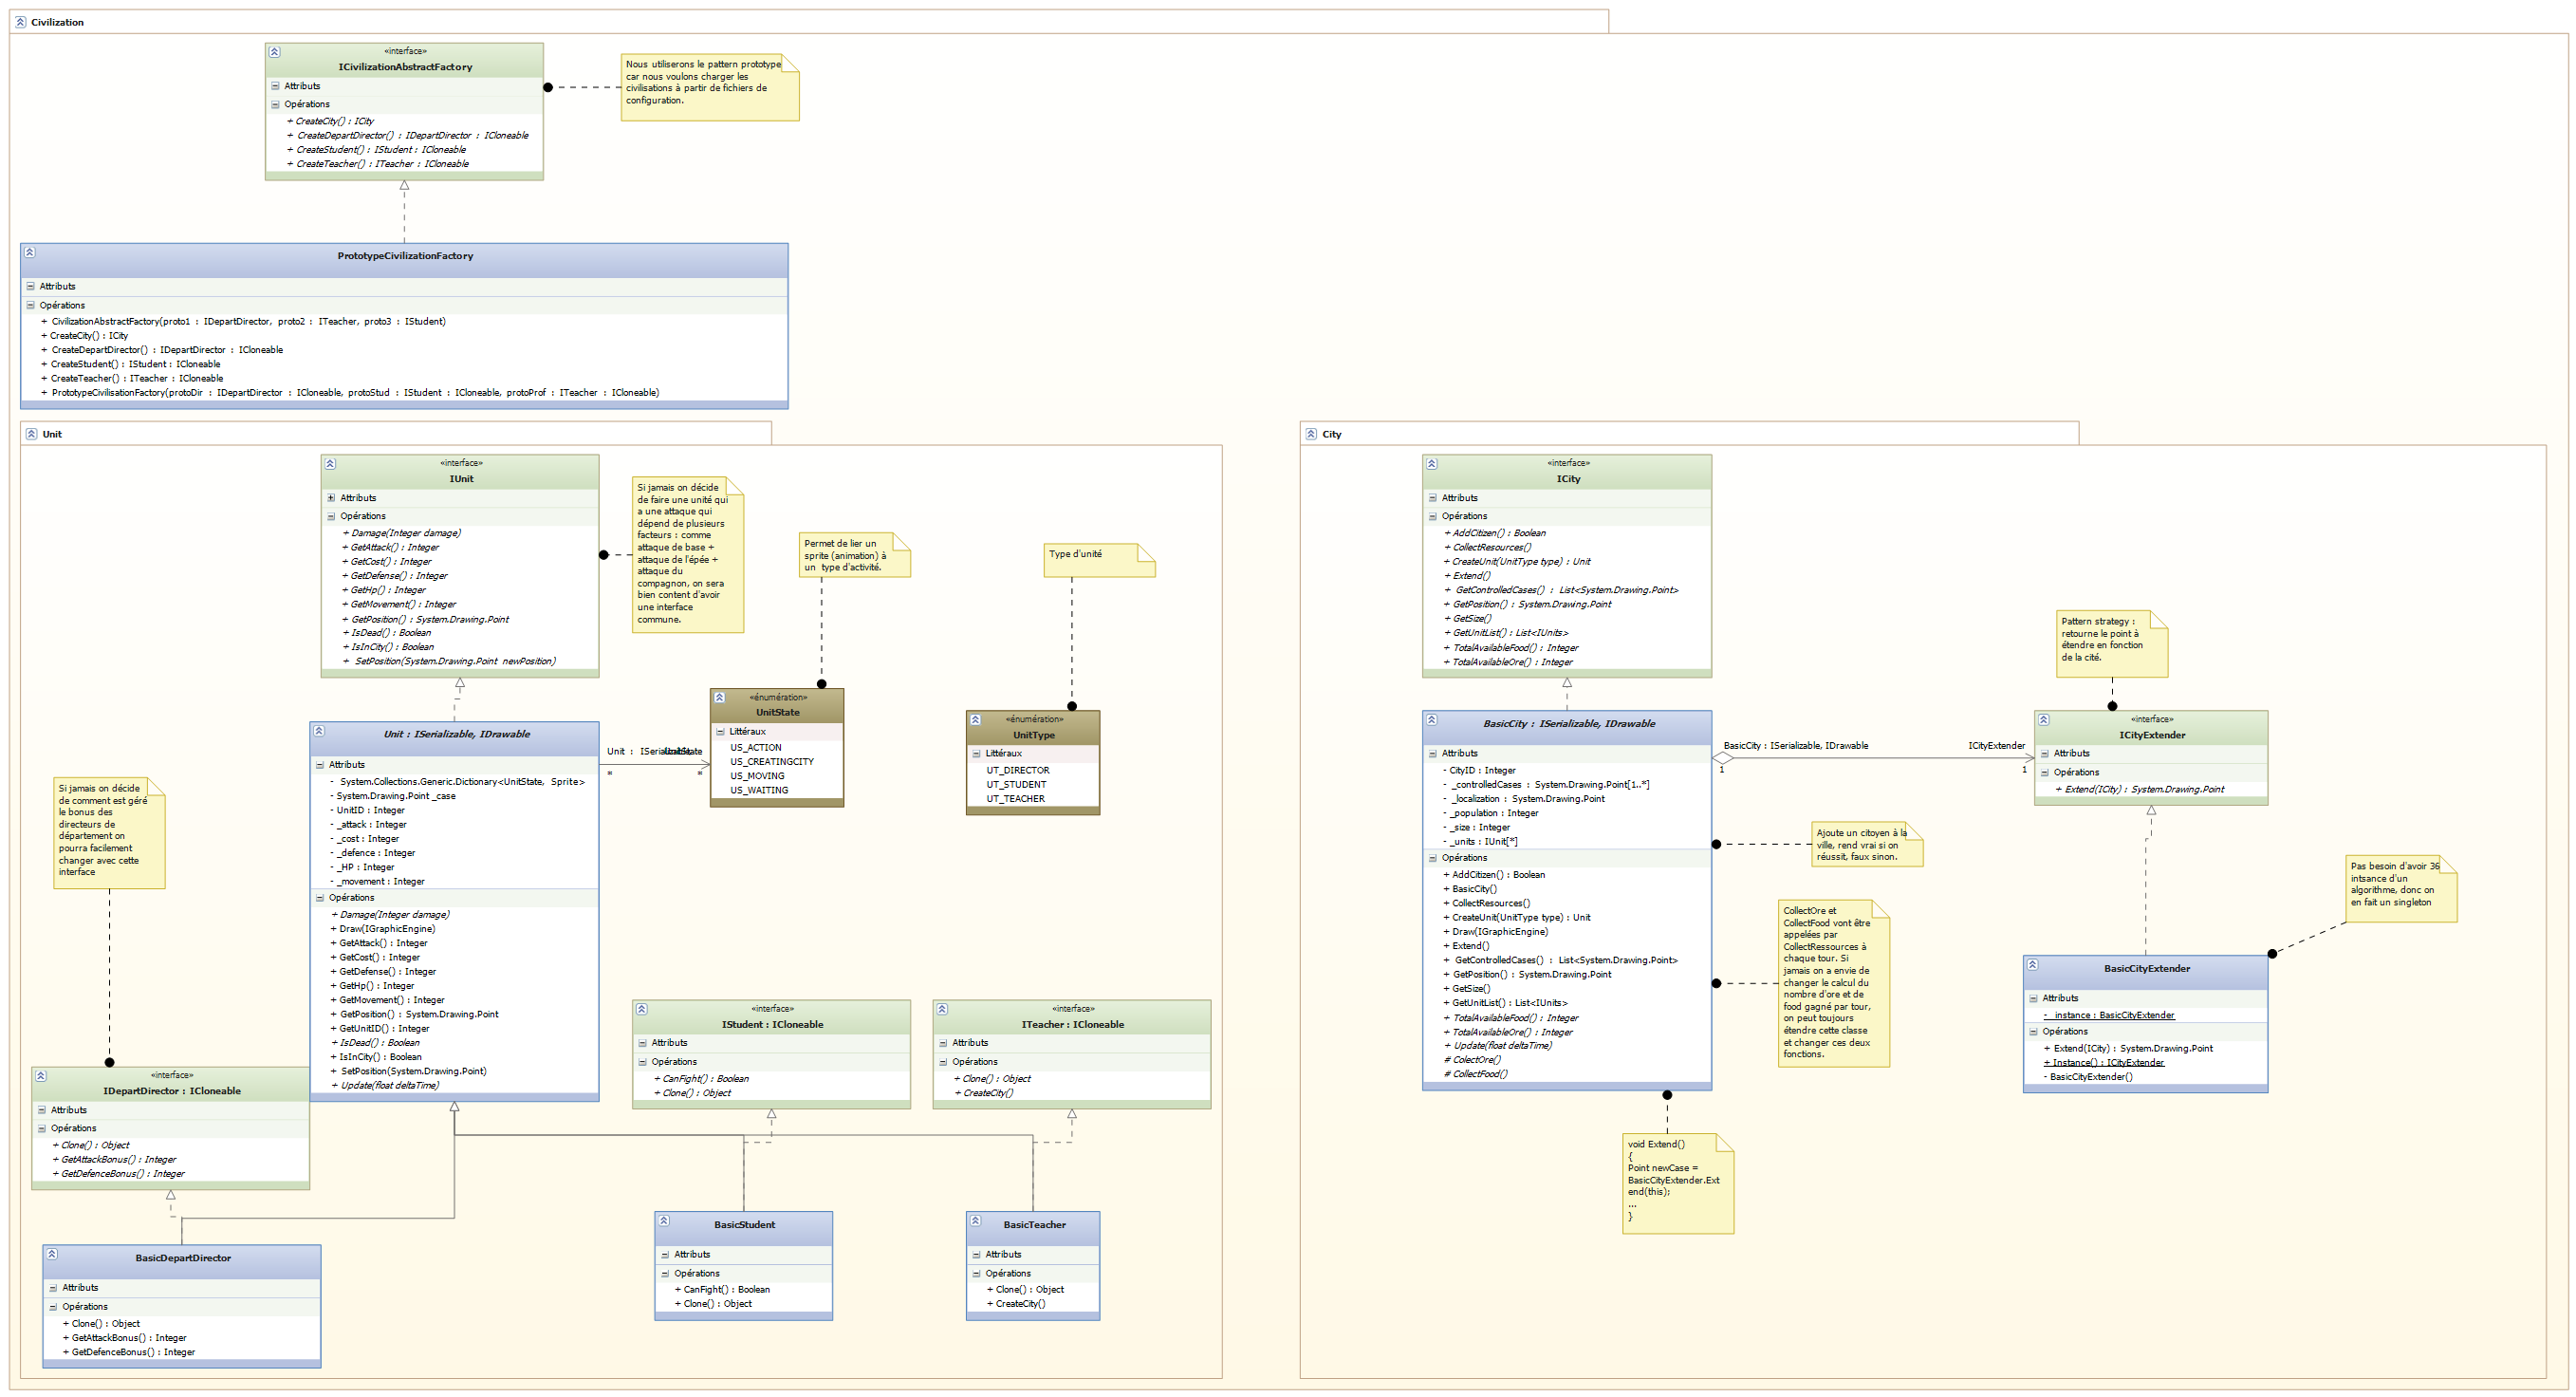
\includegraphics[width=\textwidth]{civ.png}
    \caption{Civilization.}
    \label{civ}
\end{center}
\end{figure}

\begin{figure}
    \begin{center}  
    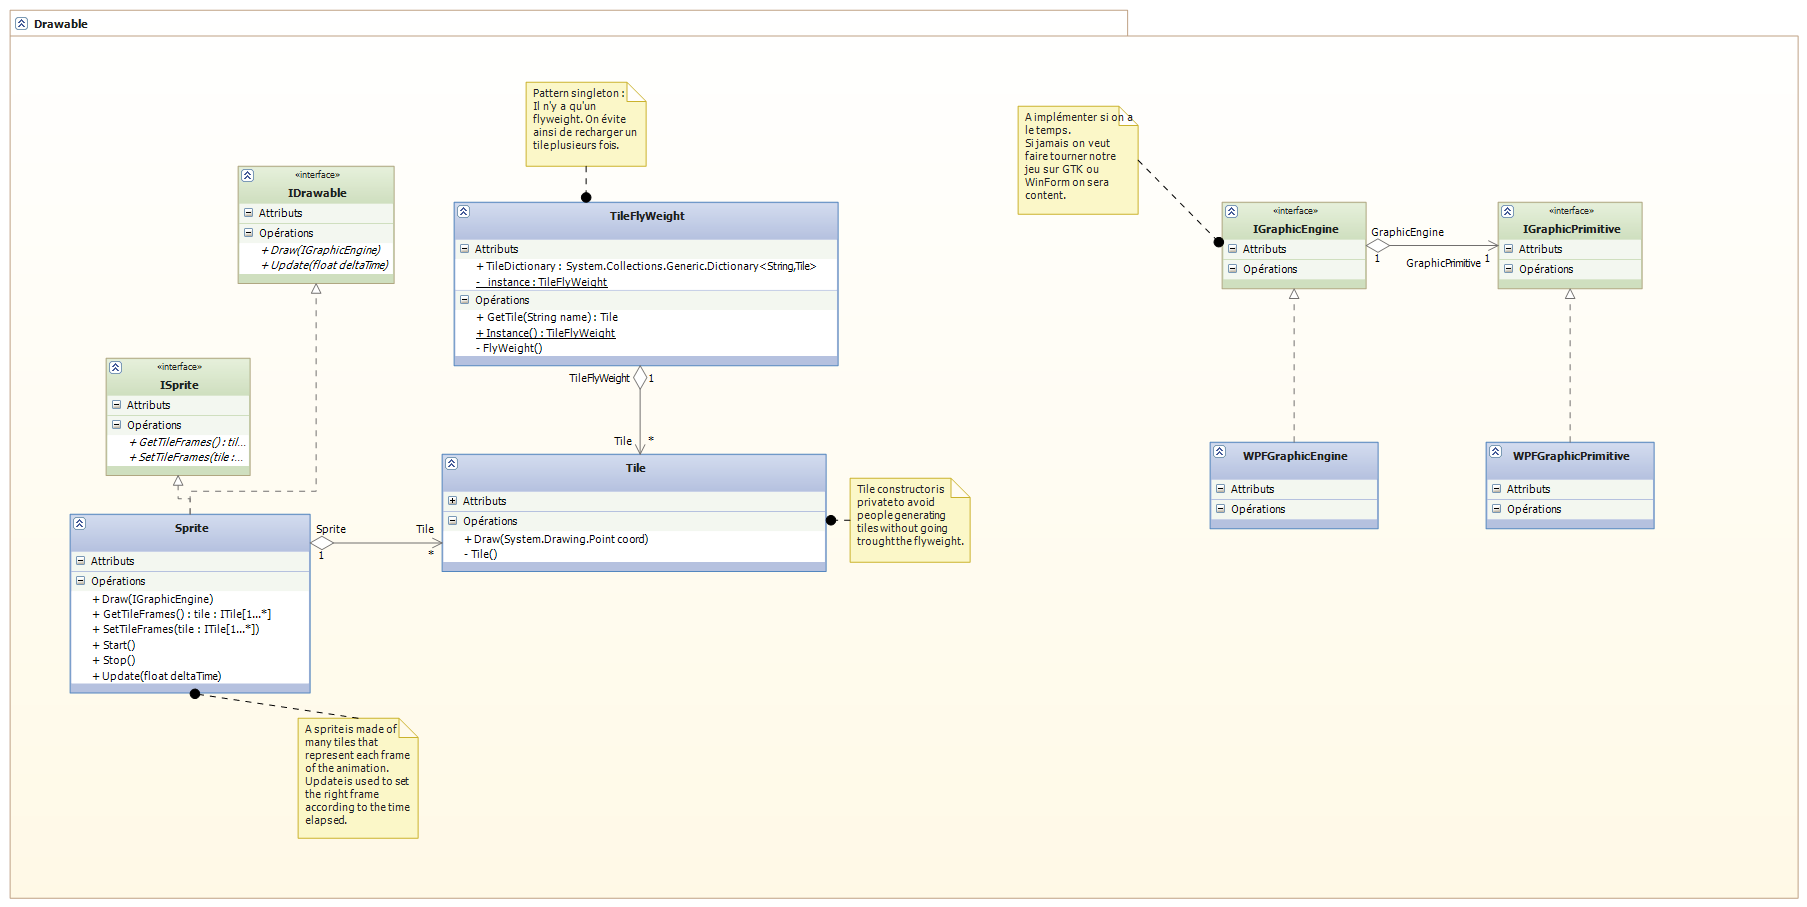
\includegraphics[width=\textwidth]{view.png}
    \caption{View.}
    \label{view}
\end{center}
\end{figure}

\begin{figure}
    \begin{center}  
    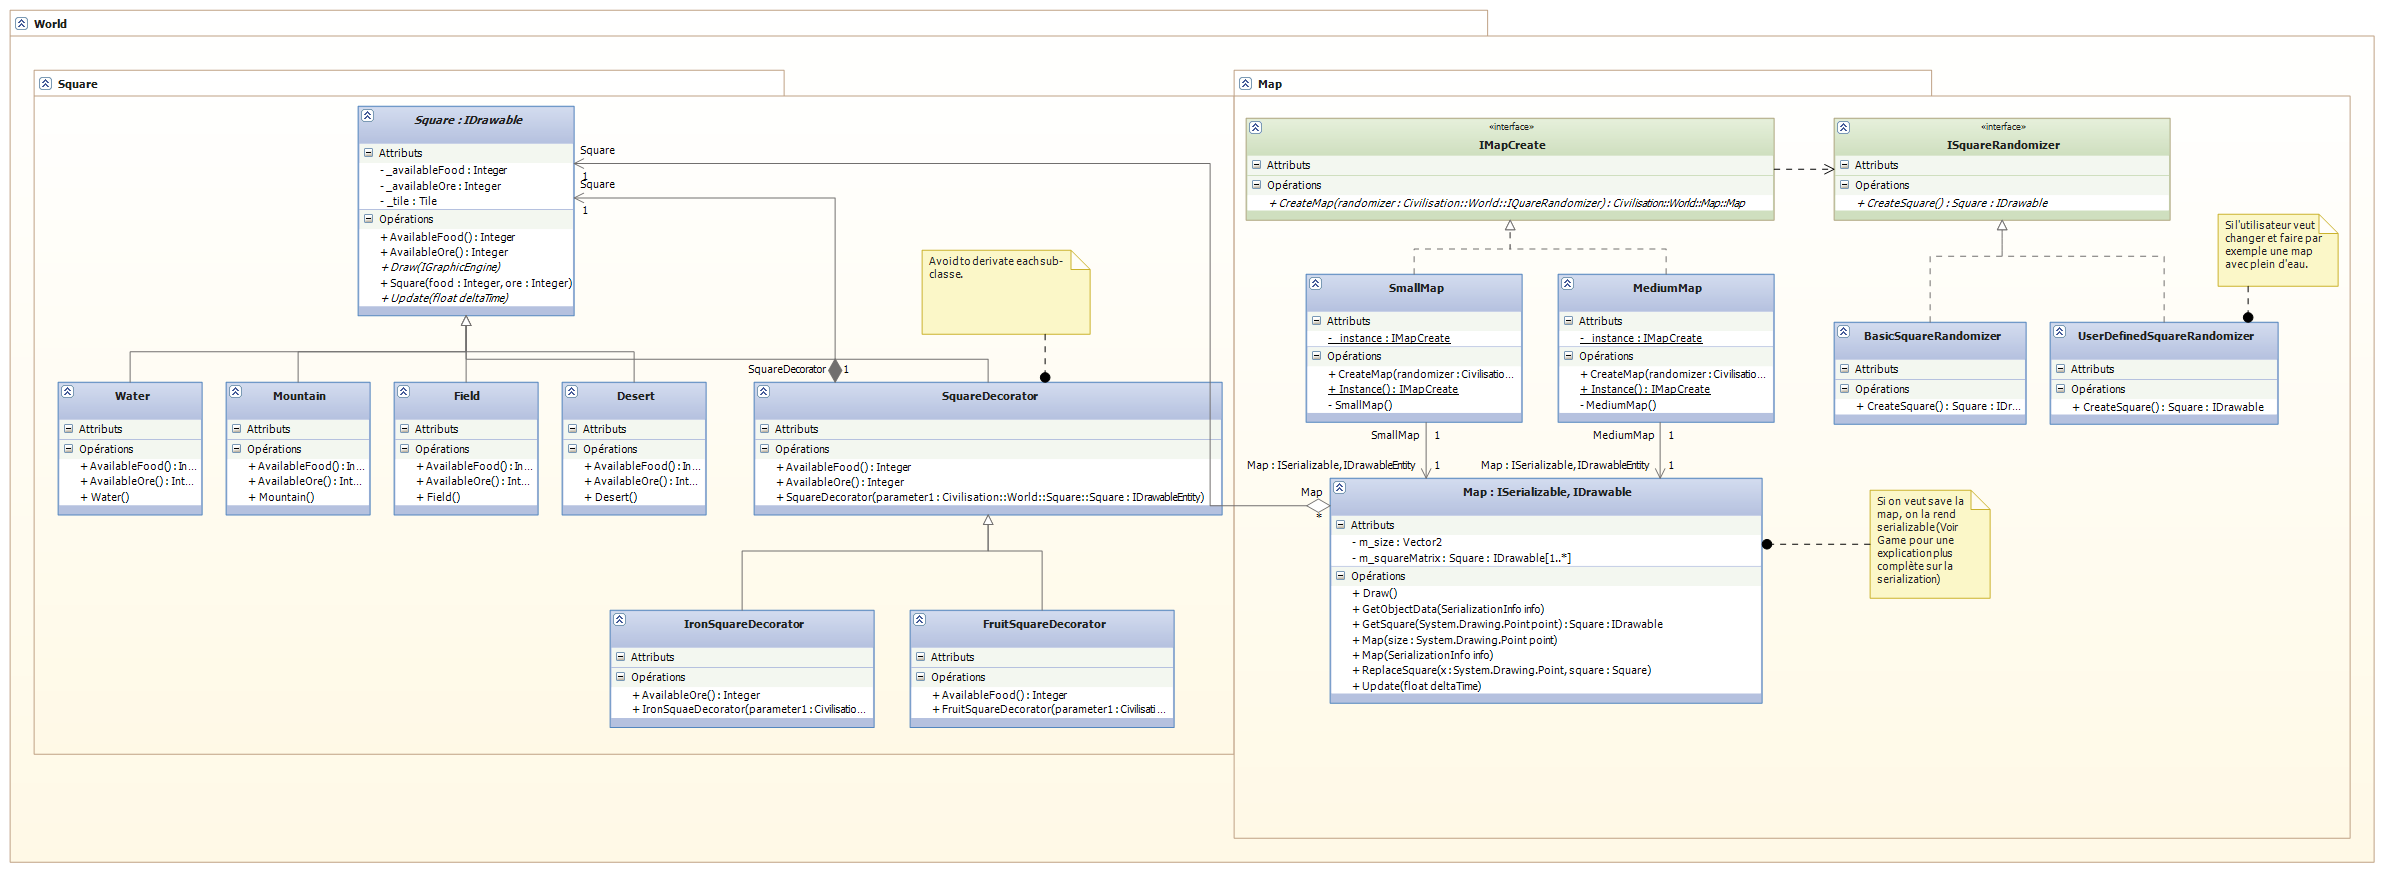
\includegraphics[width=\textwidth]{world.png}
    \caption{World.}
    \label{world}
\end{center}
\end{figure}

\begin{figure}
    \begin{center}  
    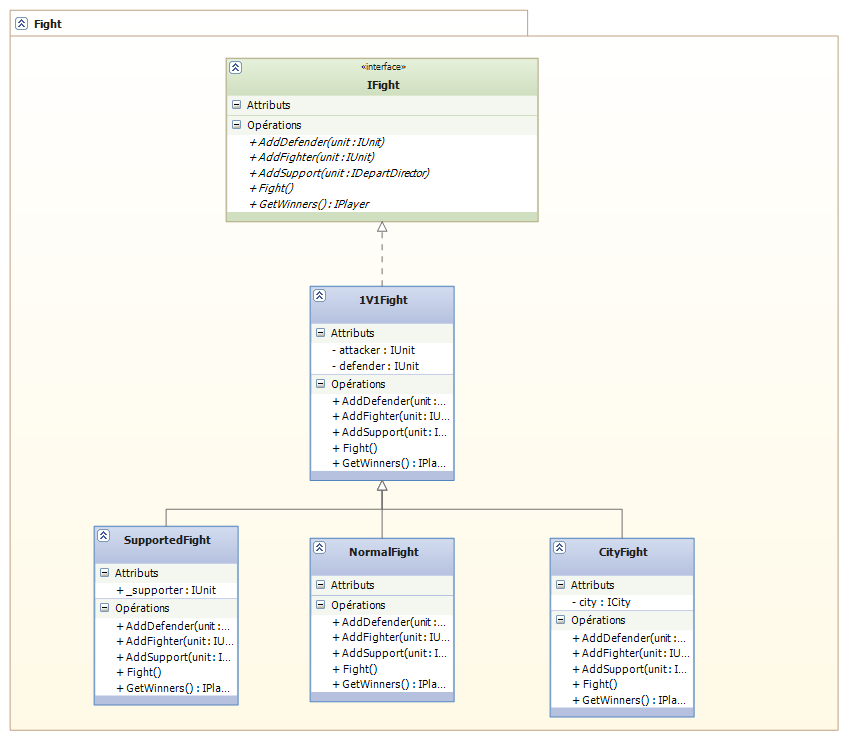
\includegraphics[width=\textwidth]{fight.png}
    \caption{Fight.}
    \label{fight}
\end{center}
\end{figure}

\begin{figure}
    \begin{center}  
    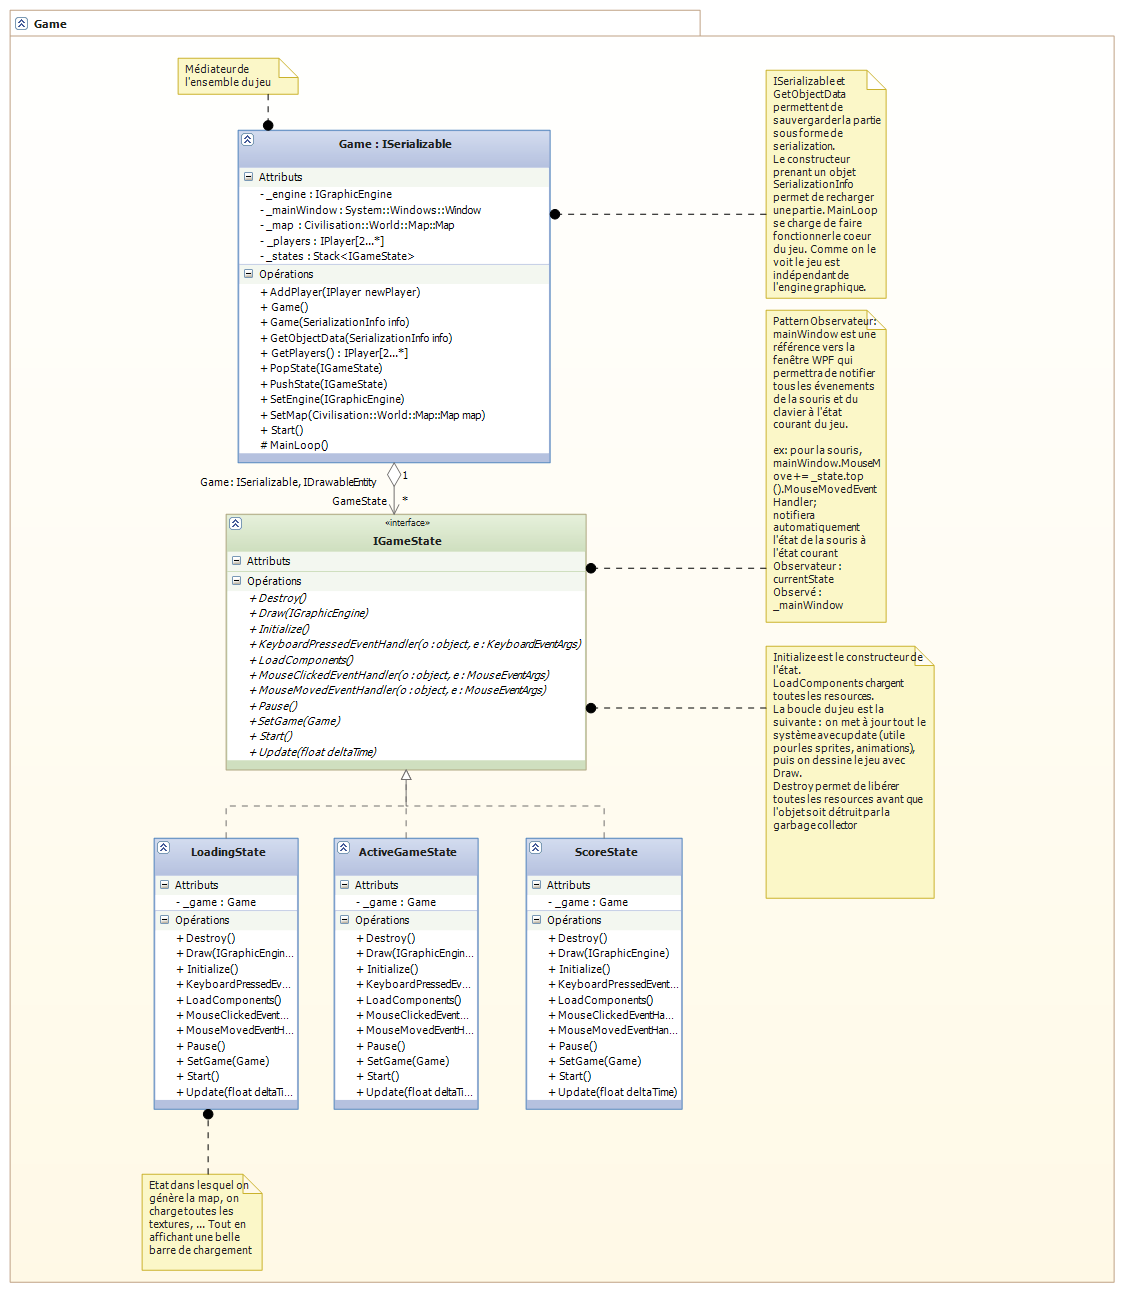
\includegraphics[width=\textwidth]{game.png}
    \caption{Game.}
    \label{game}
\end{center}
\end{figure}

\begin{figure}
    \begin{center}  
    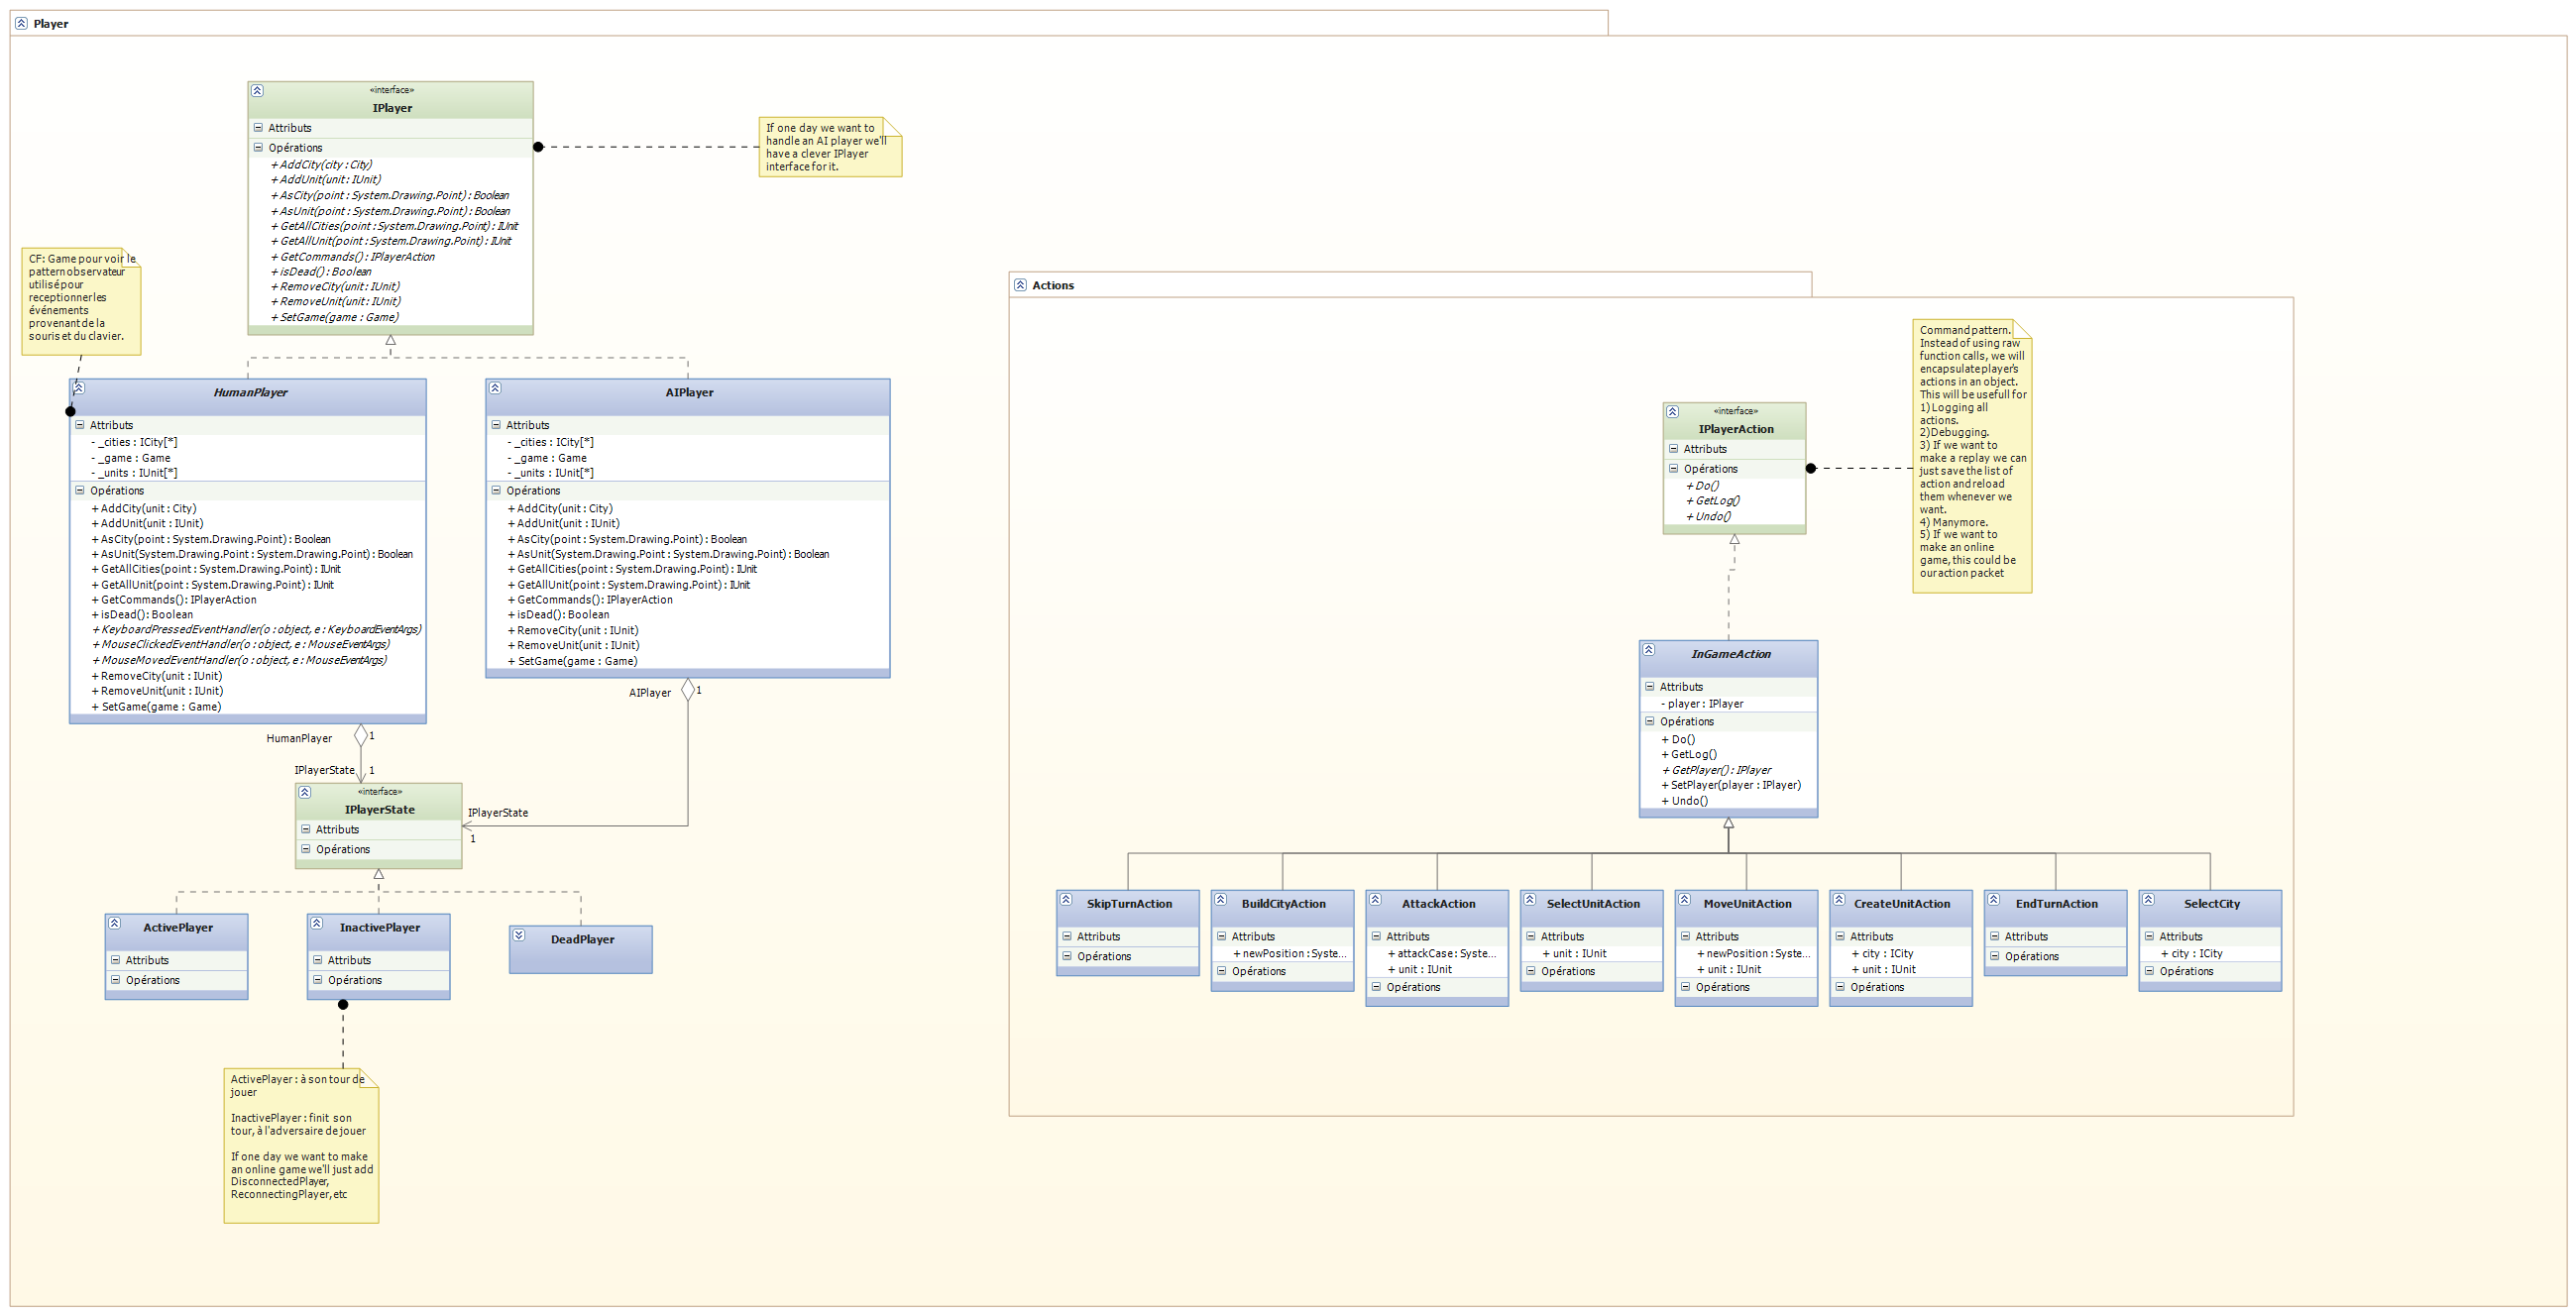
\includegraphics[width=\textwidth]{player.png}
    \caption{Player.}
    \label{player}
\end{center}
\end{figure}

\begin{figure}
    \begin{center}  
    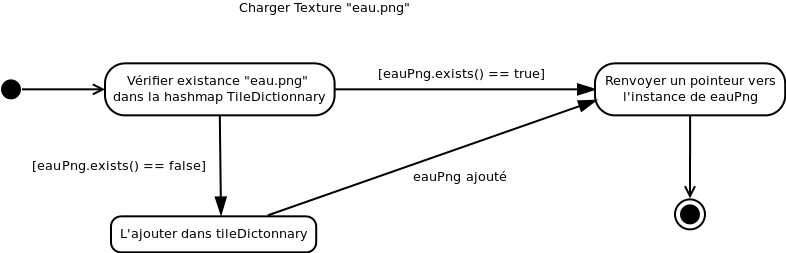
\includegraphics[width=\textwidth]{flyWeight.png}
    \caption{FlyWeight.}
    \label{flyweight}
\end{center}
\end{figure}

\begin{figure}
    \begin{center}  
    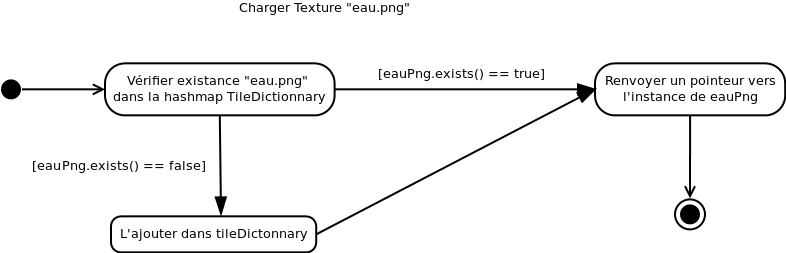
\includegraphics[width=\textwidth]{dep.png}
    \caption{Deplacement d'une unité.}
    \label{dep}
\end{center}
\end{figure}

\begin{figure}
    \begin{center}  
    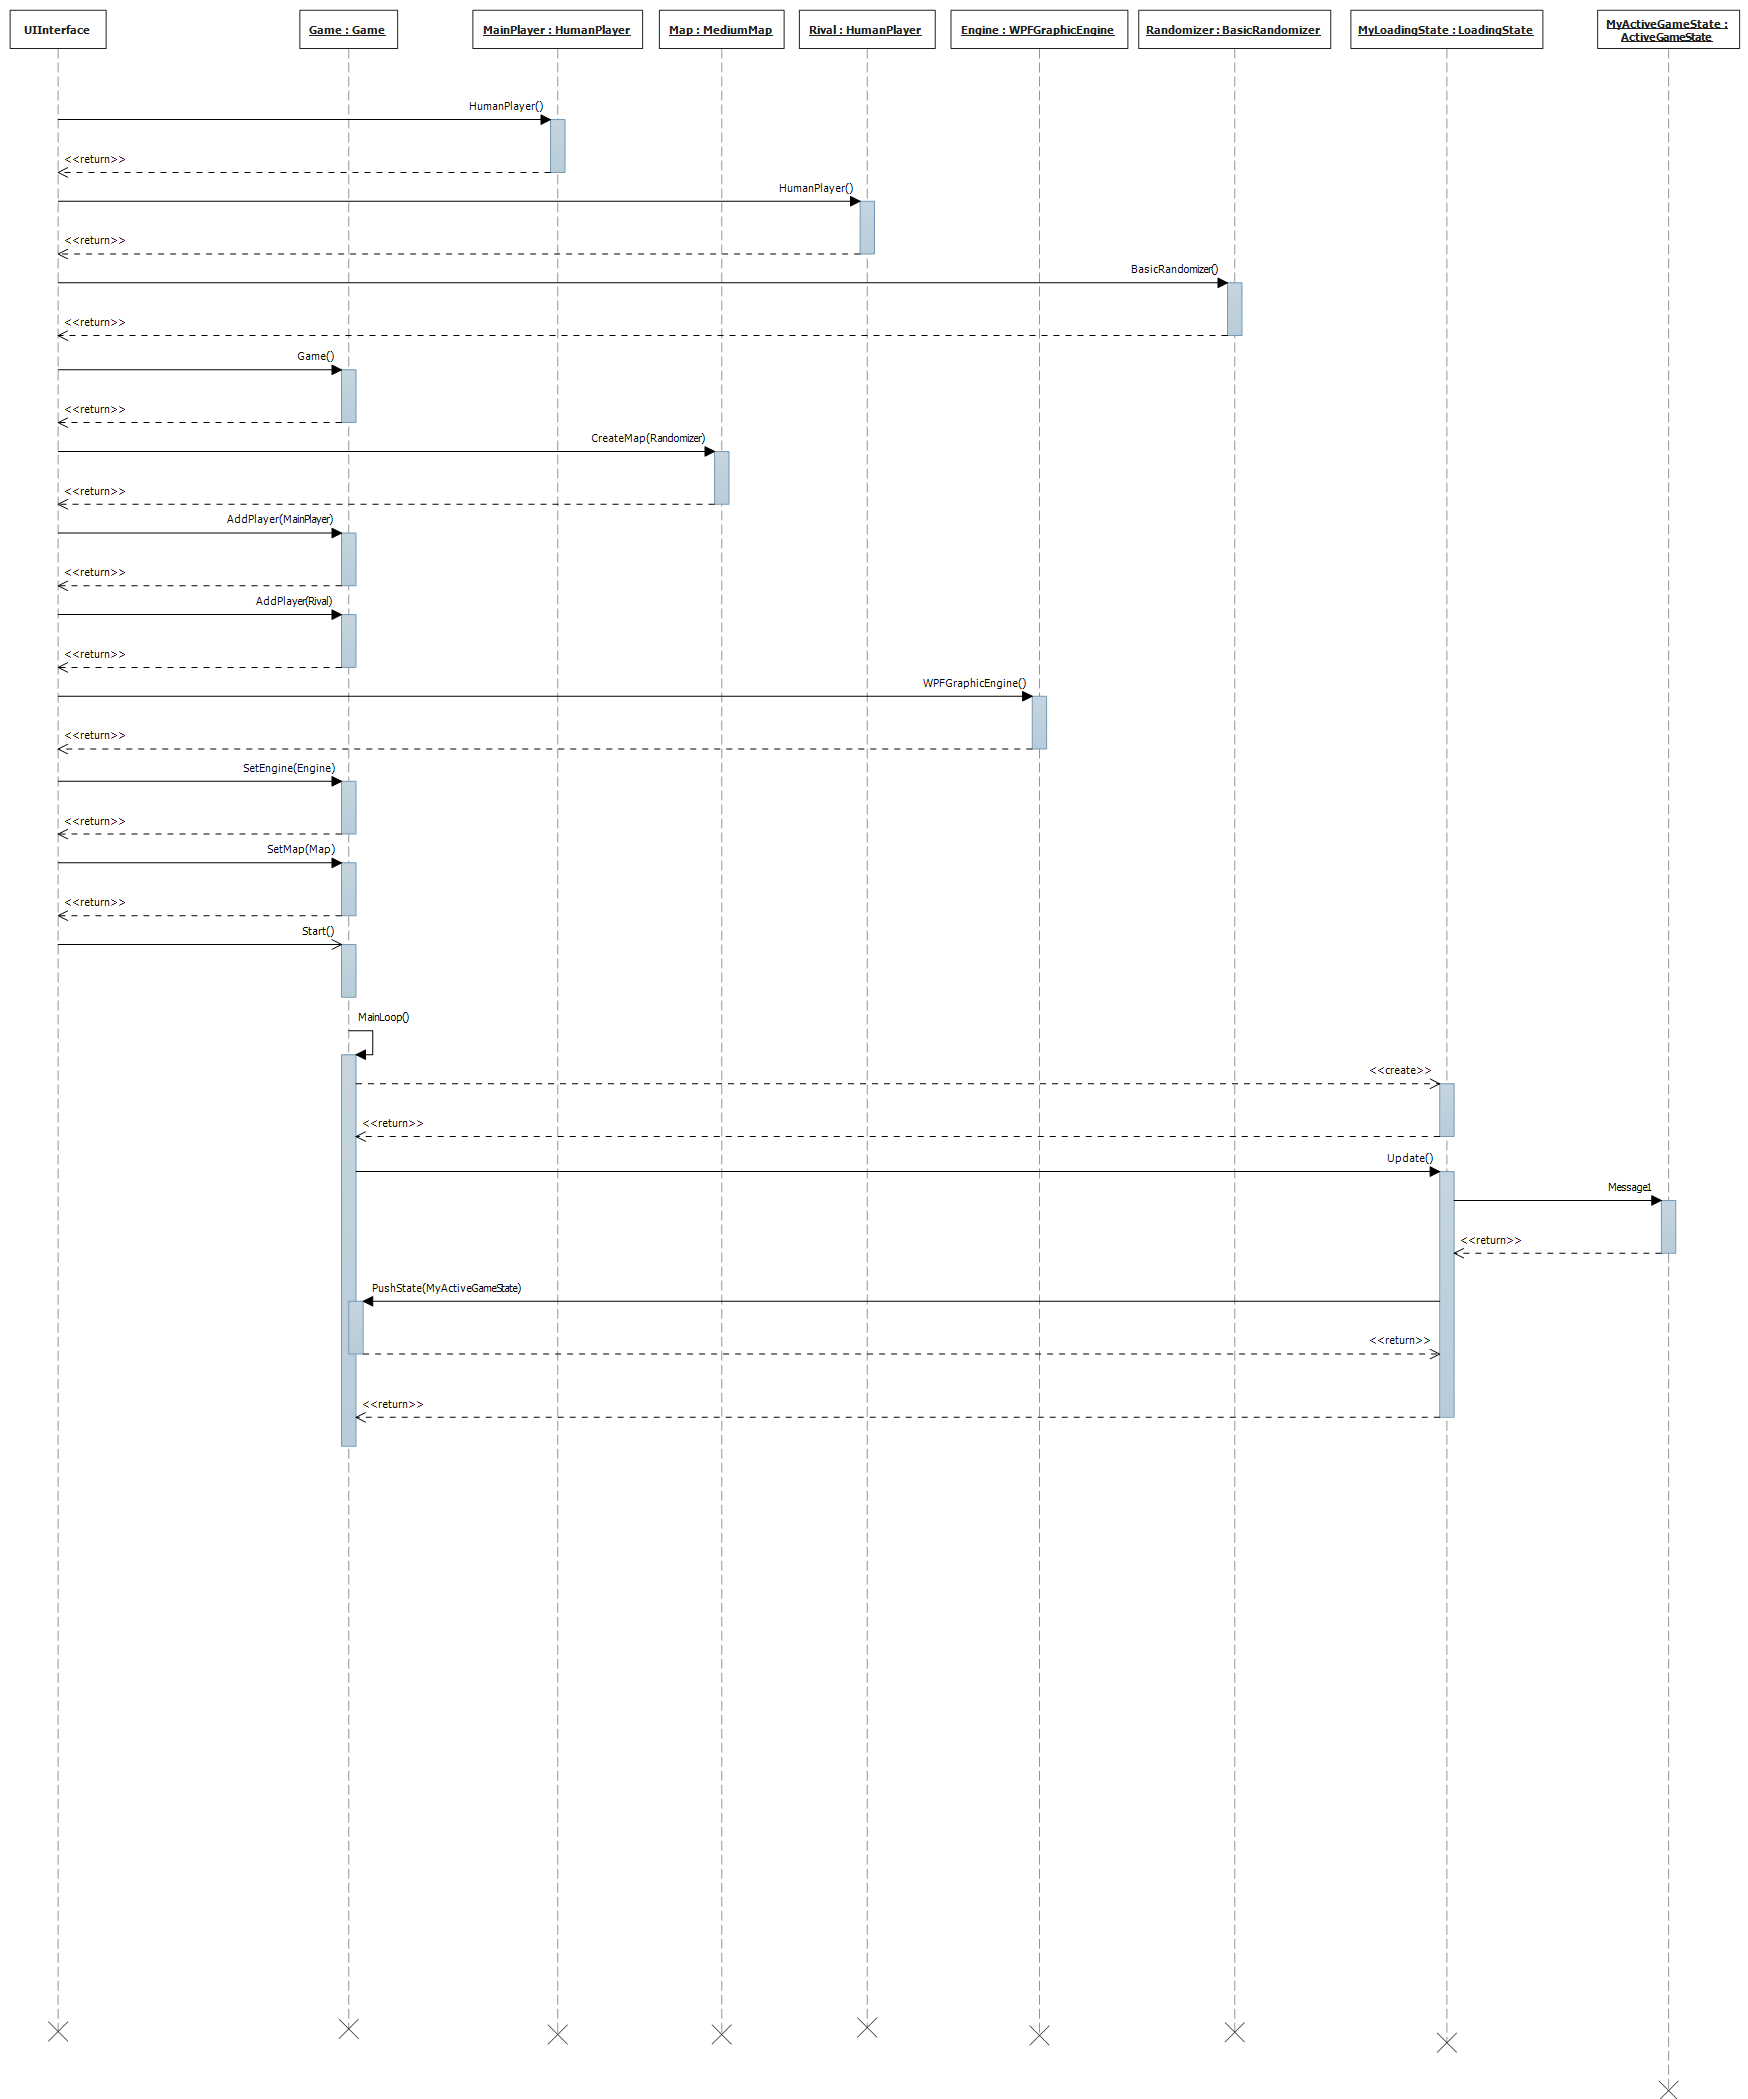
\includegraphics[width=\textwidth]{lancement.png}
    \caption{Lancement d'une partie.}
    \label{lancement}
\end{center}
\end{figure}

\begin{figure}
    \begin{center}  
    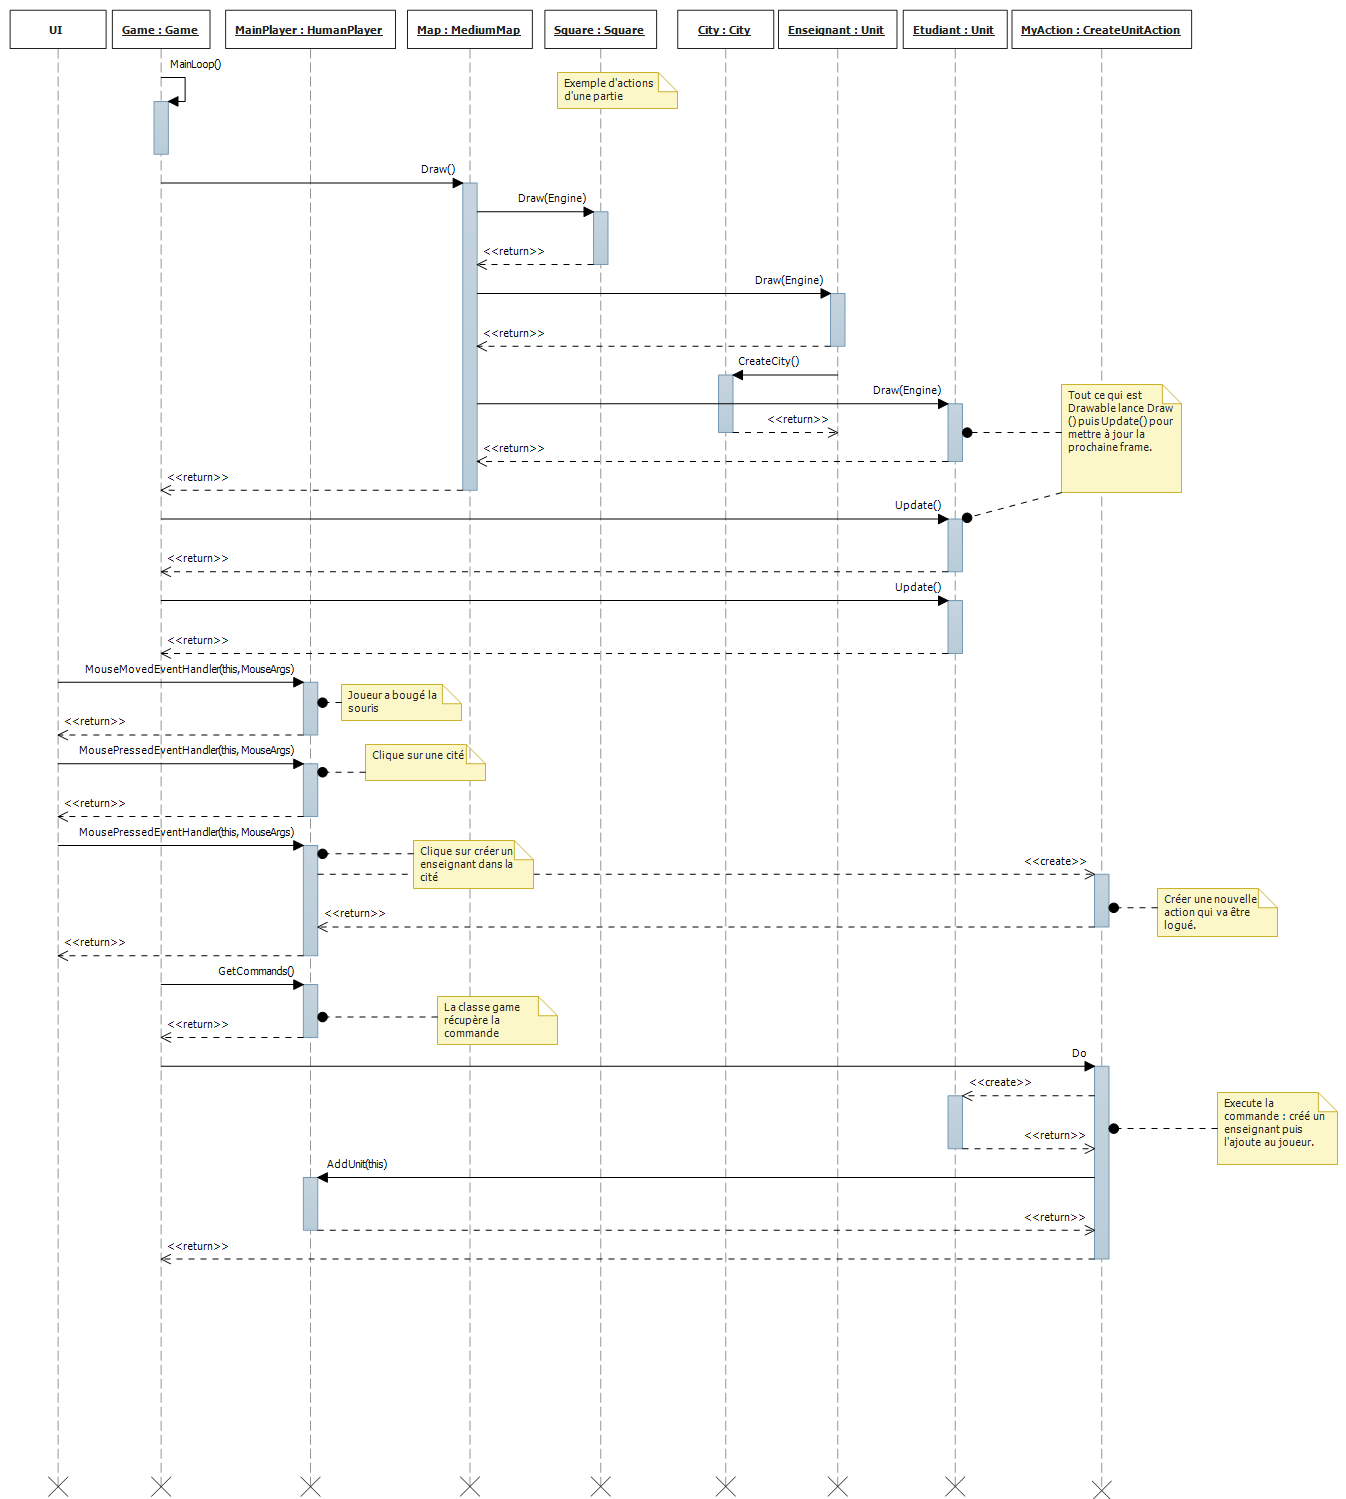
\includegraphics[width=\textwidth]{frame.png}
    \caption{Une itération dans la MainLoop.}
    \label{frame}
\end{center}
\end{figure}



































\end{document}
